\section{Техническое задание}
\subsection{Основание для разработки}

Полное наименование системы: <<Программная система для визуализации объектов в трёхмерном пространстве>>.

Основанием для разработки является приказ ректора ЮЗГУ от <<17>> апреля 2025 г. №1828-с <<О направлении (допуске) на практику>>.

\subsection{Цель и назначение разработки}

Основной целью преддипломной практики является разработка программной системы (графического движка) для визуализации трёхмерных данных в реальном времени для ООО <<Предприятие ВТИ-Сервис>>.

Посредством разработки данного движка планируется решить ряд технических задач, стоящих перед компанией. Цели разработки можно разделить на две основные группы: технические и практические.

Задачами данной разработки являются:

\begin{enumerate}
    \item Реализация базовых компонентов графического конвейера на основе OpenGL.
    \item Создание кроссплатформенного решения с использованием SDL2.
    \item Разработка системы управления шейдерами и текстурами.
    \item Реализация системы камеры.
    \item Создание базовых геометрических примитивов.
    \item Разработка формата файлов сцены.
    \item Разработка системы загрузки и отображения сцен.
\end{enumerate}

\subsection{Требования к программной системе}

\subsubsection{Требования к интерфейсу пользователя}

Интерфейс пользователя должен быть максимально простым для концентрации на визуализации трёхмерных объектов. Один из вариантов внешнего вида окна программы представлен на рисунке \ref{interface:image}.

\begin{figure}[ht]
\center{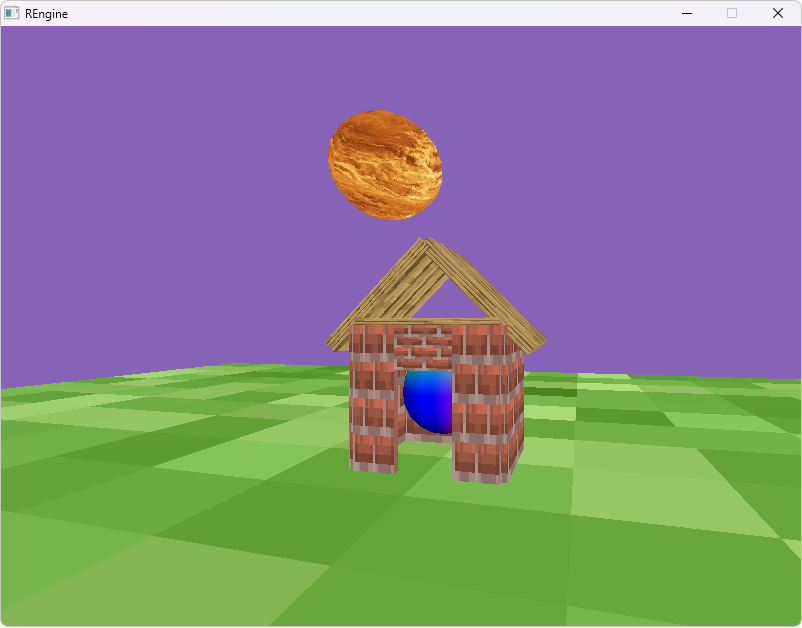
\includegraphics[width=1\linewidth]{screenshot.png}}
\caption{Окно программы}
\label{interface:image}
\end{figure}

\subsubsection{Функциональные требования}

Для разрабатываемого графического движка была построена модель, отражающая основные сценарии его использования в корпоративной среде.

Данная модель помогает выявить ключевые точки интеграции движка с существующими информационными системами предприятия, а также определить роли пользователей и взаимодействие с внешними системами. Для описания сценариев используется унифицированный язык визуального моделирования UML.

Диаграмма вариантов использования описывает функциональное назначение разрабатываемой системы. Она является исходным концептуальным представлением системы в процессе ее проектирования и разработки. Проектируемая система представляется в виде ряда прецедентов, предоставляемых системой актерам или сущностям, которые взаимодействуют с системой. Актером или действующим лицом является сущность, взаимодействующая с системой извне (например, человек, техническое устройство). Прецедент служит для описания набора действий, которые система предоставляет актеру.

На основании анализа предметной области в программе должны быть реализованы следующие функции:

\begin{enumerate}
    \item Создание и модификация сцен из узлов с трёхмерными объектами.
    \item Отображение сцен.
    \item Загрузка и применение текстур к объектам.
    \item Работа с камерой, изменение положения, углов камеры, угла зрения.
    \item Освещение сцены в реальном времени (метод Фонга) любым количеством точечных источников света.
    \item Изменение положения, цвета источников света.
    \item Возможность загрузки пользовательских вершинных и фрагментных шейдеров.
\end{enumerate}

\subsubsection{Описание API движка}

Движок предоставляет программный интерфейс (API) для создания и управления 3D-сценами. Основные компоненты API:

\begin{itemize}
    \item \texttt{Window} - управление окном приложения;
    \item \texttt{Renderer} - рендеринг сцены;
    \item \texttt{Scene} - представление 3D-сцены;
    \item \texttt{InputHandler} - обработка пользовательского ввода;
    \item \texttt{Mesh} - геометрические примитивы;
    \item \texttt{Shader} - управление шейдерами;
    \item \texttt{Texture} - работа с текстурами.
\end{itemize}

\paragraph{Инициализация приложения}

Для инициализации приложения необходимо создать окно и настроить рендерер, после чего запустить основной цикл и корректно завершить работу движка. Для этого применяются функции из файла \texttt{Window.h}.

\begin{lstlisting}[language=C++, caption=Пример инициализации приложения]
// Создание окна (2-й и 3-й аргументы - ширина и высота окна соответственно)
if (REngine::createWindow("Название окна", 800, 600) != 0) {
    // Обработка ошибки
}

// Основной цикл приложения
REngine::mainLoop();

// Завершение работы
REngine::destroyWindow();
\end{lstlisting}

\paragraph{Работа со сценой}

Сцена содержит коллекцию объектов, источников света и камеру. Для определения сцены используется структура \texttt{Scene}, которая содержит объекты -- \texttt{SceneNode}, направленный свет -- \texttt{DirLight}, вектор точечных источников света -- \texttt{PointLight}, камеру -- \texttt{CameraNode}.

Каждый объект имеет следующие параметры: указатель на объект -- \texttt{mesh}, позицию -- \texttt{position}, поворот -- \texttt{rotation}, масштаб -- \texttt{scale}, степень блеска -- \texttt{shininess}, искажение текстуры -- \texttt{distort}, путь к текстуре -- \texttt{texturePath}, путь к текстуре отражений -- \texttt{specularPath}.

\begin{lstlisting}[language=C++, caption=Пример работы со сценой]
// Создание сцены
REngine::Scene scene;

// Настройка камеры
scene.camera.position = glm::vec3(0.0f, 0.0f, 3.0f);
scene.camera.rotation = glm::vec3(0.0f, 0.0f, 0.0f);
scene.camera.fov = 45.0f;

// Настройка освещения
scene.skyColor = glm::vec3(0.63f, 0.63f, 0.85f);
scene.dirLight = {
    .direction = glm::vec3(-0.2f, -1.0f, -0.3f),
    .ambient = glm::vec3(0.2f),
    .diffuse = glm::vec3(0.5f),
    .specular = glm::vec3(1.0f)
};
scene.pointLights = {
    {
        .position = glm::vec3(1.0f, 1.0f, 1.0f),
        .constant = 1.0f,
        .linear = 0.09f,
        .quadratic = 0.032f,
        .ambient = glm::vec3(0.2f),
        .diffuse = glm::vec3(0.5f),
        .specular = glm::vec3(1.0f)
    }
};

// Добавление объекта в сцену
REngine::SceneNode node;
node.mesh = new REngine::CubeMesh();
node.position = glm::vec3(0.0f, 0.0f, 0.0f);
node.rotation = glm::vec3(0.0f, 0.0f, 0.0f);
node.scale = glm::vec3(1.0f);
node.shininess = 32.0f;
node.distort = false;
node.texturePath = "textures/box.png";
node.specularPath = "textures/box_specular.png";
scene.nodes.push_back(node);

// Установка сцены в движок
REngine::renderer->setScene(&scene);
\end{lstlisting}

\paragraph{Обработка ввода}

API предоставляет гибкую систему обработки пользовательского ввода, реализованную в классе \texttt{InputHandler}.

Взаимодействия с клавишами клавиатуры обрабатываются с помощью функций \texttt{setKeyDownCallback}, \texttt{setKeyUpCallback}, \texttt{setKeyHoldCallback}, которые принимают код клавиши и функцию обратного вызова, которая будет вызвана при нажатии на клавишу. Нажатия на кнопки мыши аналогично обрабатываются с помощью функций \texttt{setMouseButtonDownCallback}, \texttt{setMouseButtonUpCallback}, движение мыши обрабатывается с помощью функции \texttt{setMouseMotionCallback}, а прокрутка колесика мыши обрабатывается с помощью функции \texttt{setMouseWheelCallback}.

\begin{lstlisting}[language=C++, caption=Пример настройки обработки ввода]
// Обработка нажатия клавиши
REngine::InputHandler::setKeyDownCallback(SDLK_F1, [&wireframeMode]() {
    // Отображение контура объектов
    wireframeMode = !wireframeMode;
});

// Обработка движения мыши
REngine::InputHandler::setMouseMotionCallback([&scene](int x, int y, int xrel, int yrel) {
    // Вращение камеры при движении мыши
    auto& camera = scene.camera;
    camera.rotation.y += xrel * 0.1f;
    camera.rotation.x += yrel * 0.1f;
});

// Обработка прокрутки колесика мыши
REngine::InputHandler::setMouseWheelCallback([&scene](int x, int y) {
    // Изменение поля зрения камеры
    float newFov = scene.camera.fov - y * 2.0f;
    if (newFov > 1.0f && newFov < 179.0f) {
        scene.camera.fov = newFov;
    }
});
\end{lstlisting}

\paragraph{Изменение элементов сцены}

С помощью пользовательской обработки ввода можно изменять элементы сцены, такие как параметры камеры, положение объектов, цвета источников света и любые другие параметры.

\begin{lstlisting}[language=C++, caption=Пример изменения параметров сцены]
REngine::InputHandler::setKeyHoldCallback(SDLK_UP, [&scene](float deltaTime) {
    // Изменение положения объекта
    scene.nodes[0].position += glm::vec3(0.0f, 0.1f * deltaTime, 0.0f);
});

REngine::InputHandler::setKeyDownCallback(SDLK_r, [&scene]() {
    // Изменение цвета освещения
    scene.dirLight.diffuse = glm::vec3(1.0f, 0.0f, 0.0f);
});
\end{lstlisting}

\paragraph{Использование шейдеров}

Для загрузки пользовательских шейдеров необходимо указать путь к ним через метод \texttt{setShader}. При необходимости указания uniform-переменных, можно использовать методы \texttt{setVec3}, \texttt{setVec4}, \texttt{setMat4} и другие, доступные в классе \texttt{Shader}.

\begin{lstlisting}[language=C++, caption=Пример настройки шейдеров]
// Установка шейдеров из файлов
REngine::renderer->setShader(
    "shaders/vertex.glsl",
    "shaders/fragment.glsl"
);

// Получение указателя на шейдер
Shader* shader = REngine::renderer->getShader();

// Установка uniform-переменных
shader->use();
shader->setVec3("viewPos", camera.position);
shader->setFloat("time", SDL_GetTicks() / 1000.0f);
\end{lstlisting}

\paragraph{Загрузка текстур}

Текстуры загружаются автоматически при добавлении объекта в сцену через поля \texttt{texturePath} и \texttt{specularPath}. При отсутствии текстуры движок генерирует монотонную текстуру: белую для обычной и серую для отражений.

\begin{lstlisting}[language=C++, caption=Пример загрузки текстур]
// Добавление объекта с текстурой
REngine::SceneNode texturedNode;
texturedNode.mesh = new REngine::CubeMesh();
texturedNode.texturePath = "textures/wood.png";
texturedNode.specularPath = "textures/wood_specular.png"; // Необязательно
scene.nodes.push_back(texturedNode);
\end{lstlisting}

\subsection{Нефункциональные требования к программной системе}

\subsubsection{Требования к программному обеспечению}

Для реализации разрабатываемого движка должны использоваться языки программирования C++ и GLSL, компилятор GCC и система сборки CMake.

Для запуска и работы с движком требуется использование компьютера под управлением 64-битной операционной системы Windows 7 (или выше) или Linux.

\subsubsection{Требования к аппаратному обеспечению}

Клиентское оборудование должно иметь центральный процессор с частотой ядра не менее 1 ГГц и поддержкой SSE2, а также видеокарту с поддержкой OpenGL 3.3 или выше. Объём оперативной памяти -- 512 ГБ.

Доступ к сети Интернет не требуется.

\subsection{Требования к оформлению документации}

Разработка программной документации и программного изделия должна производиться согласно ГОСТ 19.102-77 и ГОСТ 34.601-90. Единая система программной документации.
